When building new products, it is important to know the target audience. Here, a tool was to be designed that could aid educators in teaching programming to students. Thus, it was important to investigate what kind of tool the educators wanted to use in their work, since a tool that isn't needed will not be used.

\subsection{Interviews}
Some of the more experienced educators in the field that also work at \LTU{} were asked to participate in interviews. These interviews consisted of some 15--20 questions regarding the way they teach, what tools they have used, what issues they face in every-day teaching and what help they would appreciate from on-line tools. Additionally, some educators that had already done previous work on gamification were interviewed about the subject at length, yielding some useful insights into the field.

Primarily, the directions that were taken from the interviews was that:
\begin{itemize}
\item Internal motivation is better than external motivation; the latter can be used to kick-start studies, but if there is no internal motivation, the student won't go on studying once the external motivation wears off.
\item Quickly increasing the difficulty makes students fail their studies, become demotivated and drop out. Instead, increase difficulty in small increments.
\item Tools that are hard to use; expensive or otherwise time-consuming tend to find little acceptance.
\item Adding context to an assignment makes a world of difference.
\end{itemize}

\subsection{Literature studies}
In order to obtain a greater understanding of what gamification elements would work best for the system to be developed a group was formed to study papers and other literature on the subject. Aside from finding inspiration for game elements to introduce to the system, finding research on how gamifictaion affect the performance and motivation of test subjects could be valuable.

While most of the practical examples of gamification used in education found were from informal sources, some research papers examining the effects gamification might have on motivation and learning were found. While most research show promising results Dicheva et al.~\cite{ref:dicheva} mentions that more empirical studies are needed to determine the effects of gamified learning elements on intrinsic and extrinsic motivation. A study conducted by Deci et al.~\cite{ref:deci} suggests that extrinsic rewards might undermine intrinsic motivation. In order to increase motivation of students Uhr et al.~\cite{ref:uhr} mentions some recommendations and guidelines teachers should aim for then applying gamification to education: feedback should be quick and positive, tasks should be adapted to skill level, there should be different paths to achieving the goal, and the activity should be encouraged despite failures.

The literature studies showed that there is still much research needed to determine the effects of gamification in education. This made us realize it might be of interest to have the system to be developed support tests useful in gamification research. When considering what game elements should be added to the system it was found that progress should always use positive measurements, and tasks should be available for different skill levels to challenge the students appropriately and maintin motivation. Different paths to achieve the goal lets students choose the challenges that are most interesting to them. Having students compete for ranks on a leaderboard could appeal to some competative students, but might discourage those with low scores.

\subsection{Workshop}
\subsubsection{Planning}
As part of the pre-study, it was planned from the start of the project to host a workshop. A workshop is an interactive session in which participants work together on solving issues through discussion and brainstorming\cite{workshop}. 

A subgroup of the project members were responsible for planning and hosting the workshop. The planning consisted of brainstorming sessions and a consulting session with the project owner for advice on how to manage a workshop. An important question that was discussed in the brainstorming process was what the actual purpose of the workshop should be. It was decided on holding the workshop with the second out of two purposes:
\begin{itemize}  
    \item Try out game mechanics on the participants to see which mechanics should be included in the product.
    \item Find out from the participants what features the product should have and mockups of the suggested system. 
\end{itemize}

To elicit information in the workshop in accordance to the purpose of the workshop, three workshop scenarios were designed. The idea behind the scenarios is to have the participants discuss freely on certain issues that are relevant to the product. Short description of the three scenarios (for full information see Chapter~\ref{sec:workshop}):
\begin{itemize}  
    \item \textbf{Scenario 1:} Put the participants in the role of a student having to complete complete cumbersome programming assignments, think of a system that would make this more appealing.
    \item \textbf{Scenario 2:} Put the participants in the role of a teacher which years later holds the same course. Further develop and/or limit the system.
    \item \textbf{Scenario 3:} User-interface mockups of the system.
\end{itemize}
    
\subsubsection{Hosting}
Invitations were sent to students, teachers and employees at the University Pedagogy Centre, all from \LTU{}. There were 12 participants in total, five of which were moderators. The participants were randomly split into two groups. They received print-outs of the scenarios and had limited time to discuss and write down ideas on post-it notes and white-boards, which would later be presented.

\begin{figure}[hb]
\centering
    \begin{subfigure}{.32\textwidth}
        \centering
        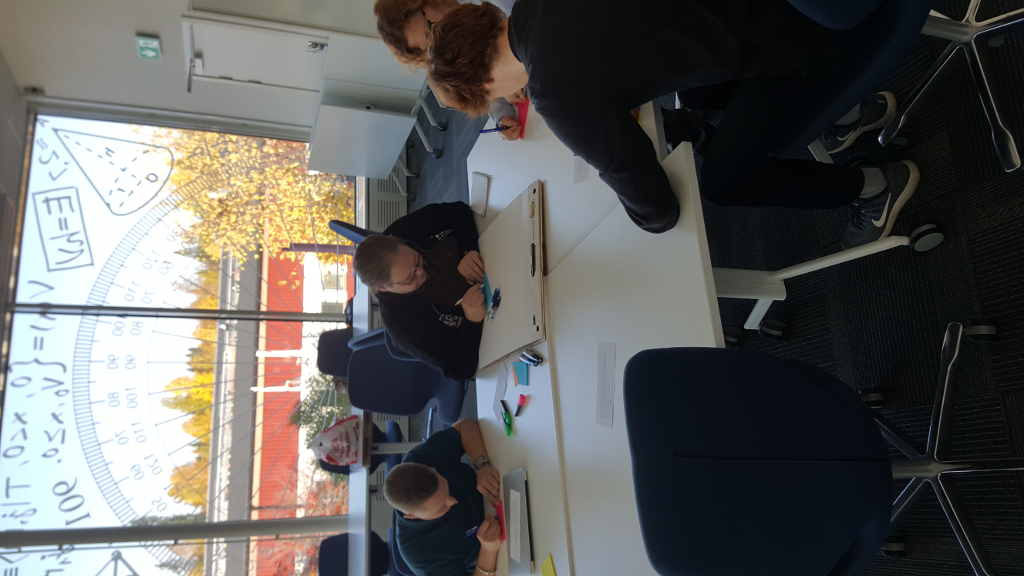
\includegraphics[width=\textwidth, angle=270, origin=c]{img/workshop1_resized.jpg}
        \label{fig:workshop1}
    \end{subfigure}
    \begin{subfigure}{.32\textwidth}
        \centering
        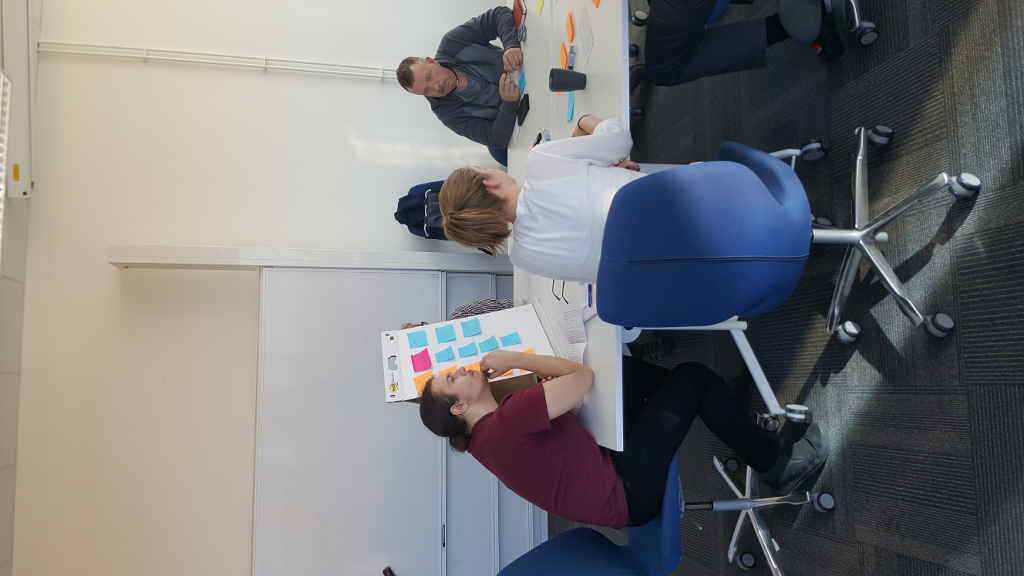
\includegraphics[width=\textwidth, angle=270, origin=c]{img/workshop2_resized.jpg}
        \label{fig:workshop2}
    \end{subfigure}
    \begin{subfigure}{.32\textwidth}
        \centering
        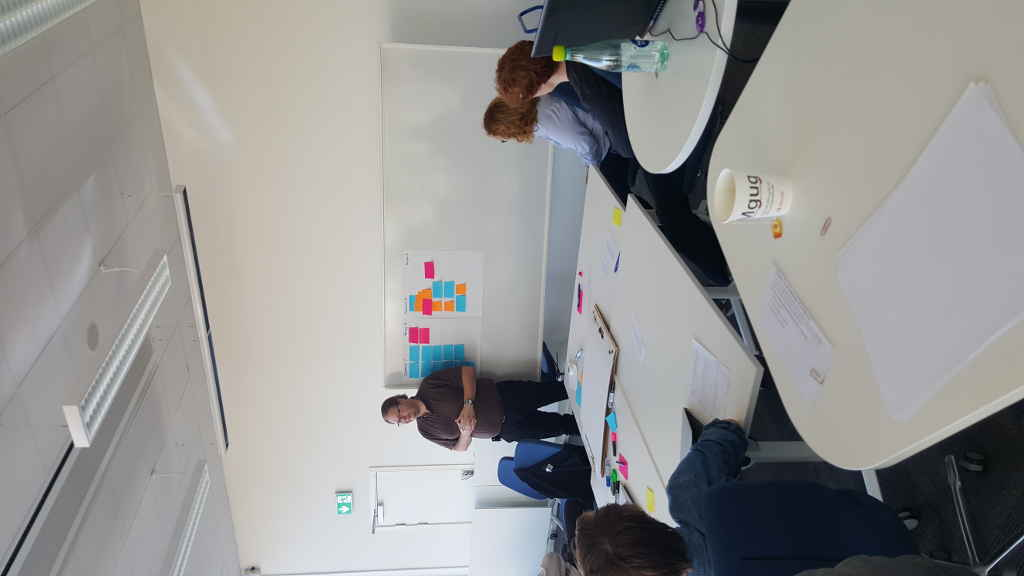
\includegraphics[width=\textwidth, angle=270, origin=c]{img/workshop3_resized.jpg}
        \label{fig:workshop3}
    \end{subfigure}
    \caption{Workshop images.}
\end{figure}

\subsubsection{Results}
Summarized results from the workshop:

\begin{itemize}
    \item Gamification elements will motivate students to perform the assignments.
    \item Social support, encourage students to cheer for one-another through collaboration.
    \item Anonymous questions so students doesn't have to be afraid to ask questions. Should generate statistics for the teacher.
    \item More direct contact between teachers and students, live-chat.
    \item Fast feedback for students when doing assignments. 
    \item Personality tests to customize gamification elements and/or UI.
    \item Students correct assignments completed by other students, and create assignments for one another.
    \item An internal knowledge-bank for the system, similar to \href{https://stackoverflow.com/}{Stackoverflow}, where students can find help with certain courses and/or assignments.
\end{itemize}

\begin{figure}[H]
\centering
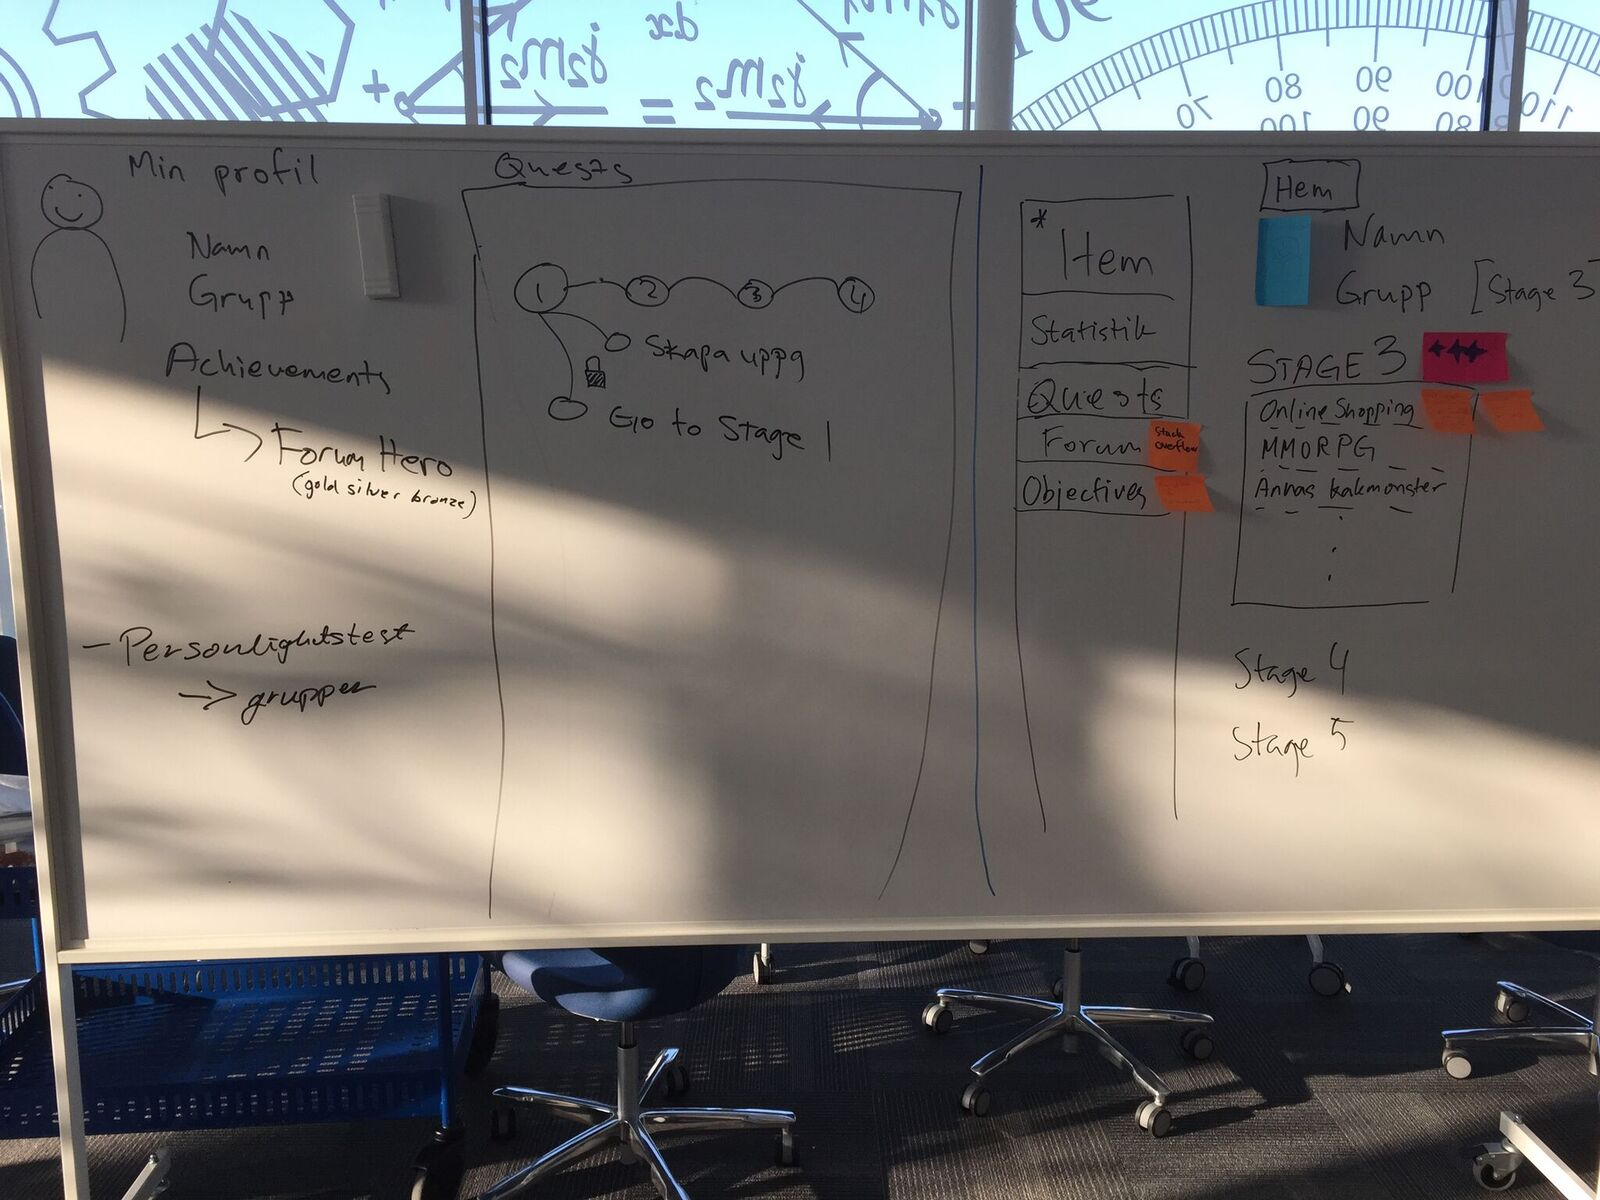
\includegraphics[width=0.8\textwidth]{img/Grupp2_Workshop_mockup.jpg}
\caption{Some notes taken by paritipants.}
\label{fig:workshop4}
\end{figure}
